\section{Общая характеристика работы}
\textbf{Актуальность темы исследования.} Изменения, происходящие в городской среде вследствие технического прогресса, требуют формирования новых методов планирования и развития инфраструктуры города для создания более комфортной жизни людей. Одной из наиболее важных сторон развития города является организация оптимальной транспортной системы города, в частности~--- системы общественного транспорта.

Несмотря на кажущуюся хаотичность перемещений жителей, все они подчиняются определенным закономерностям, связанных с масштабом и планировкой городской среды. Для принятия решений по изменению или созданию маршрутной сети города необходимо выявить эти закономерности в поведении населения, и по этим закономерностям сформировать обобщенную модель перемещения жителей внутри города, на основе которой можно будет строить и оценивать различные варианты системы городского общественного транспорта. В рамках магистерской диссертации следует разработать метод кластеризации предпочтений жителей города по перемещению для создания сети остановочных пунктов.

\textbf{Цель и задачи работы.} Целью данной работы являлась разработка метода кластеризации геораспределенных данных с учетом рельефа местности. Для достижения 
поставленной цели решались следующие задачи:
\begin{itemize}
    \item генерация псевдореалистичных данных о перемещениях жителей;
    \item разработка метрики расстояний, учитывающей рельеф местности;
    \item модификация и использование существующих алгоритмов для кластеризации геораспределенных данных, полученных из картографического сервиса OpenStreetMap, с разработанной метрикой расстояний;
    \item представление построенных кластеров на карте.
\end{itemize}

\textbf{Объектом исследования} является кластеризация предпочтений жителей города по перемещению, выраженных в виде пары точек «Пункт отправления — пункт назначения», каждая из которых содержит две координаты — широту и долготу.

\textbf{Предметом исследования} является разработка и применение методов кластеризации предпочтений жителей, учитывающих элементы рельефа местности.

\textbf{Гипотеза исследования.} Использование данных о перемещениях жителей и автоматизация построения сети остановочных пунктов и маршрутной сети позволяют построить оптимальную сеть маршрутов общественного транспорта.

\textbf{Научная новизна} работы: разработан алгоритм кластеризации на основе
k-means, использующий метрику расстояния, вычисленную с использованием
карт городской местности, позволяющую учитывать городской рельеф.

\textbf{Практическая ценность.} Данная система может быть использована:
\begin{itemize}
    \item в системах формирования сети общественного транспорта;
    \item в системах обработки географических данных.
\end{itemize}

\textbf{Публикации.} По материалам диссертации автором опубликовано 3 работы, 2 из которых представлены в рецензируемом научном журнале, входящем в перечень Высшей аттестационной комиссии. 

\textbf{Структура и объем работы.} Диссертационная работа состоит из введения, четырех глав, заключения, списка использованных источников из 49 наименований и насчитывает 99 страниц, в том числе 57 страниц основного текста, 26 рисунков, 1 таблицу и 2 приложения.

\section{Основное содержание работы}
\textbf{Во введении} обосновываются выбор темы диссертационного исследования и ее актуальность, определяются 
цели и задачи работы, объект, предмет и гипотеза исследования, формулируется научная новизна.

\textbf{В первой главе} приводятся результаты исследования предметной области. Произведен анализ общего состояния существующей проблемы в кластеризации, в том числе с учетом препятствий, и обработке геораспределенных данных. Рассмотрена литература по современным исследованиям в данной области и методам предлагаемых в них. Следует отметить, что обработка препятствий в существующих алгоритмах не производится напрямую с географическими данными~--- данные о препятствиях рассчитываются из диаграмм Воронова и Делоне, накладывая ограничения на рассматриваемые точки; либо не рассчитываются, а обход препятствий заключается в работе алгоритма, <<предполагающего>> наличие препятствий. В результате был сделан вывод, что существующие решения не приспособлены для работы с данными, получаемых из картографических сервисов, и не могут в полной мере учитывать элементы рельефа; и, как следствие, могут применяться для формирования сети остановочных пунктов в полуавтоматическом режиме, требуя вмешательства транспортного инженера.

Для оптимизации маршрутной сети общественного транспорта необходимо проанализировать большой объем данных, характеризующих численность и мобильность населения, среднее время перемещения, расположение мест приложения труда и жилых массивов. Источниками этих данных выступают статистические сборники, выписки о численности сотрудников крупных предприятий, собираемые муниципальными предприятиями общественного транспорта, информация о количестве проданных билетах на маршрутах общественного транспорта. Для сбора данных о перемещениях жителей организуется целый комплекс мероприятий по натурному подсчету пассажиропотока в подвижном составе общественного транспорта и на остановочных пунктах существующих маршрутов, а также анкетированию жителей. Такие традиционные методы являются достаточно трудоемкими, а полученные данные не в полной мере отражают динамично меняющуюся ситуацию. В связи с этим, необходимо использовать современные технологии и новые ресурсы для получения актуальных данных о предпочтениях жителей по перемещениям в городе и интенсивности пассажиропотоков. Основываясь на современных подходах к анализу данных можно получить ценную информацию для поддержки принятия решений в процессе планирования развития транспортной системы города.

\textbf{Во второй главе} рассмотрены и проанализированы существующие методы, применимые к задаче кластеризации. Подробно рассмотрено три алгоритма, которые можно применить для кластеризации геораспределенных данных, если использовать в них предложенную метрику расстояний и подобрать конкретные параметры управления под конкретные выборки. Также описан основной метод, используемый для кластеризации геораспределенных данных в данной работе, и предложенная метрика, учитывающая элементы городского рельефа.

Задачу кластеризации можно представить следующим образом:\\
Пусть \( X \)~--- входная выборка точек, полученная из географических сервисов, функция расстояния между элементами \( \rho(x, x') \), и \( k \)~--- ожидаемое число узлов (остановочных пунктов) во входной выборке. Требуется разбить выборку на \( C \)~--- \( k \) непересекающихся подмножеств элементов, называемых кластерами, таким образом, чтобы каждый кластер состоял из объектов, близких по метрике \( \rho \), а объекты разных кластеров существенно различались. При этом метрика \( \rho \) должна оценивать географическую близость элементов, учитывая рельеф городской местности.

Задача является типичной задачей машинного обучения без учителя, но имеет некоторые специфические особенности. Во-первых, стандартные применяемые метрики для решения данной задачи не подходят: необходимо учитывать особенности местности, такие как реки, овраги и балки, автомобильные и железные дороги, здания и промышленные зоны. Существуют алгоритмы, учитывающие препятствий, но они не опираются на карту местности, а хранят информацию о препятствиях в некотором абстрактном виде. Во-вторых, поскольку на выходе необходимо получить сеть остановочных пунктов, то центры рассчитываемых кластеров должны находиться на участках дорожной сети, а не в произвольной географической точке.
\begin{figure}[b!]
\vspace*{-1em}
\begin{algorithm}[H]
    \KwData{\( X \), \( k \), \( C_0 \), \( I \).}
    \KwResult{\( C \), \( L \).}
    1. \( C = C_0 \), \( L_0 = \varnothing \), \( i = 0\)\;
    2. \While{\( L != L_0\) и \( i < I \)}{
        1. \( L_0 = L \), \( A = \varnothing \), \( \mu = \varnothing \)\;
        2. \ForEach{\( x \in X \)}{
            1. \( r = \varnothing \)\;
            2. \ForEach{\( c \in C \)}{
                1. Рассчитать \( r_{xc} = \rho(x, c) \)\;
                2. \( r = r + \{ r_{xc} \} \)\;
            }
            3. \( L[x] = C[\min(r)] \)\;
            4. \( A[C[\min(r)]] = A[C[\min(r)]] + \{x\}\)\;
        }
        3. \ForEach{\( c \in C \)}{
            1. \( \mu[c] = \sum(A[c])\,/ \abs{A[c]} \)\;
            2. \( c = \mu[c] \)\;
        }
        4. \( i = i + 1 \)\;
    }
\end{algorithm}
\vspace*{-2em}
\caption{Алгоритм k-means}
\label{alg:kmeans}
\end{figure}

В качестве базового алгоритма кластеризации был выбран алгоритм k-средних ввиду его удобной расширяемости на поставленную задачу и вида входных данных, которые можно считать равномерно распределенными по рассматриваемой области, то есть в них нет четко выраженных кластерных структур.

Псевдокод алгоритма представлен на схеме~\ref{alg:kmeans}.

Предлагается два способа расчета расстояний между географическими объектами. Первый способ заключается в использовании в качестве расстояний решения обратной геодезической задачи для рассматриваемых точек (метрика <<Surface>>). Второй способ заключается в использовании в качестве расстояний длину маршрута между двумя рассматриваемыми точками (метрика <<Route>>).

Метрика Surface рассчитывает расстояние путем решения обратной геодезической задачи. Метрика Route рассчитывает расстояние между объектами по графу городских дорог.

\textbf{В третье главе} описана методология проектирования ПО, разработана методика проведения эксперимента, произведено испытание разработанных алгоритмов, а также обсуждены полученные результаты в ходе эксперимента и сделан вывод на их основе.

Предложенные алгоритмы были реализованы с использованием языка программирования Python и сервиса построения маршрутов Open Source Routing Machine (OSRM) для расчета расстояния между географическими точками по городским дорогам.
\begin{figure}[b!]
    \centering
    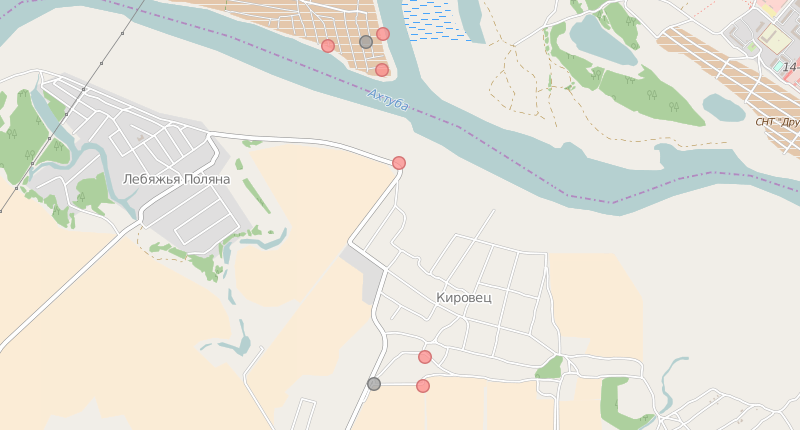
\includegraphics[width=.9\textwidth]{test_river}
    \caption{Тестовый пример <<Река>>. Красные точки обозначают объекты выборки, черные~--- начальные центры кластеров}
    \label{img:river}
    \vspace*{-2em}
\end{figure}

\begin{figure}[t!]
    \centering
    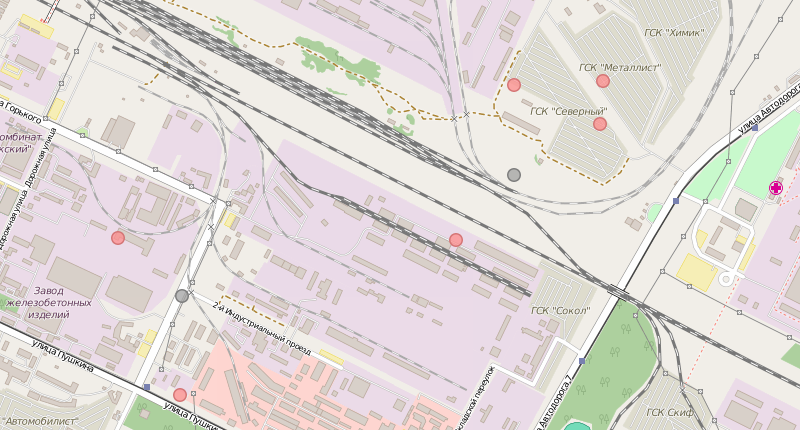
\includegraphics[width=.9\textwidth]{test_railway}
    \caption{Тестовый пример <<Железная дорога>>. Красные точки обозначают объекты выборки, черные~--- начальные центры кластеров}
    \label{img:railway}
    \vspace*{-1ex}
\end{figure}

В качестве тестовых примеров для проверки расчета расстояний было сделано две тестовые выборки: <<Река>>, представленная на рис.~\ref{img:river}, и <<Железная дорога>>, представленная на рис.~\ref{img:railway}, между объектами которых располагаются река и железная дорога соответственно.

При кластеризации выборок из этих примеров с использованием обычных метрик объекты, между которыми находится препятствие, попадают в один кластер: рис.~\ref{img:river-sur}, \ref{img:railway-sur}.
\begin{figure}[b!]
    \centering
    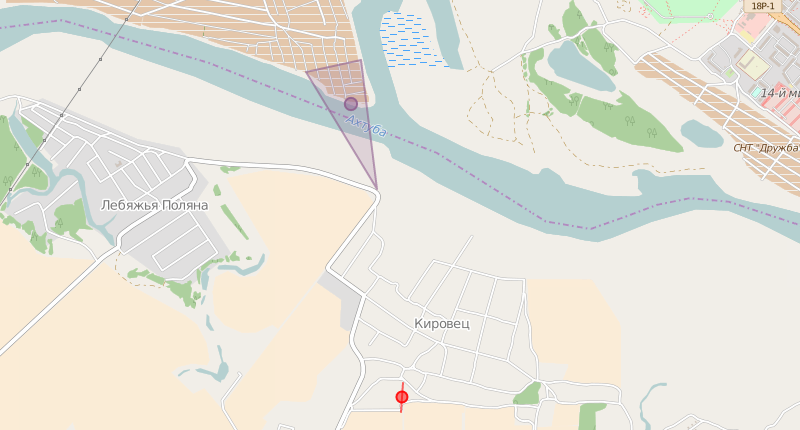
\includegraphics[width=.9\textwidth]{river_surface}
    \caption{Кластеризация выборки из тестового примера <<Река>> с метрикой Surface}
    \label{img:river-sur}
    \vspace*{-1em}
\end{figure}

\begin{figure}[t!]
    \centering
    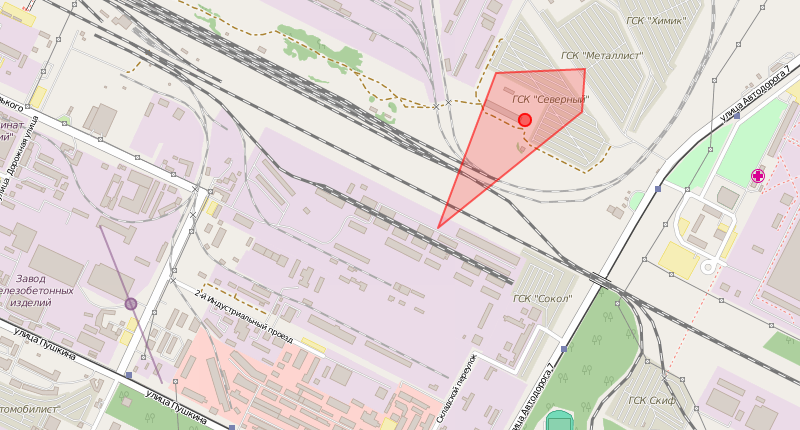
\includegraphics[width=.9\textwidth]{railway_surface}
    \caption{Кластеризация выборки из тестового примера <<Железная дорога>> с метрикой Surface}
    \label{img:railway-sur}
    \vspace*{-1ex}
\end{figure}

При кластеризации выборок из этих примеров с использованием метрики Route объекты, разделенные препятствиями, попадают в разные кластеры: рис.~\ref{img:river-route}, \ref{img:railway-route}.

\begin{figure}[ht!]
    \centering
    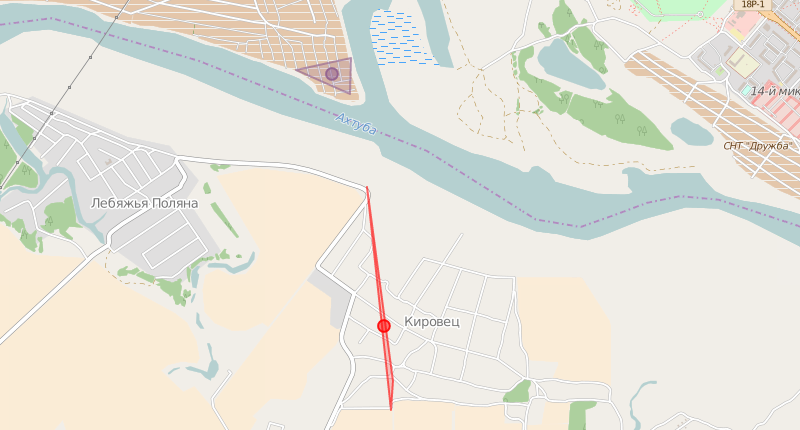
\includegraphics[width=.9\textwidth]{river_route}
    \caption{Кластеризация выборки из тестового примера <<Река>> с метрикой Route}
    \label{img:river-route}
    \vspace*{-1ex}
\end{figure}

\begin{figure}[ht!]
    \centering
    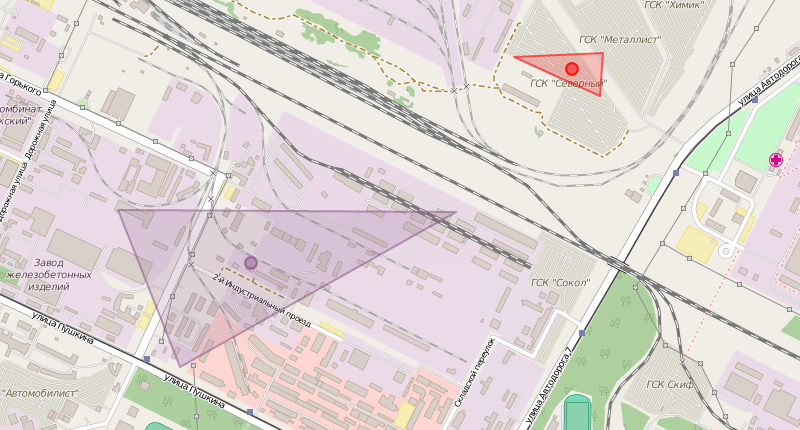
\includegraphics[width=.9\textwidth]{railway_route}
    \caption{Кластеризация выборки из тестового примера <<Железная дорога>> с метрикой Route}
    \label{img:railway-route}
    \vspace*{-1ex}
\end{figure}

Метрика Route построена на получении данных о расстоянии между точками по графу городской дорожной сети. Для получения этих данных используется сервис построения маршрутов Open Source Routing Machine с профилем работы для автомобиля.

Для тестирования работы алгоритма и метрик была сгенерирована псевдореалистичная выборка данных (<<Main>>), состоящая из 12 тысяч точек. Кластеризация проводилась с идентичным начальным набором из 125 кластеров. Результаты работы представлены на рис.~\ref{img:full-surface}, \ref{img:full-route}.
\begin{figure}[ht!]
    \centering
    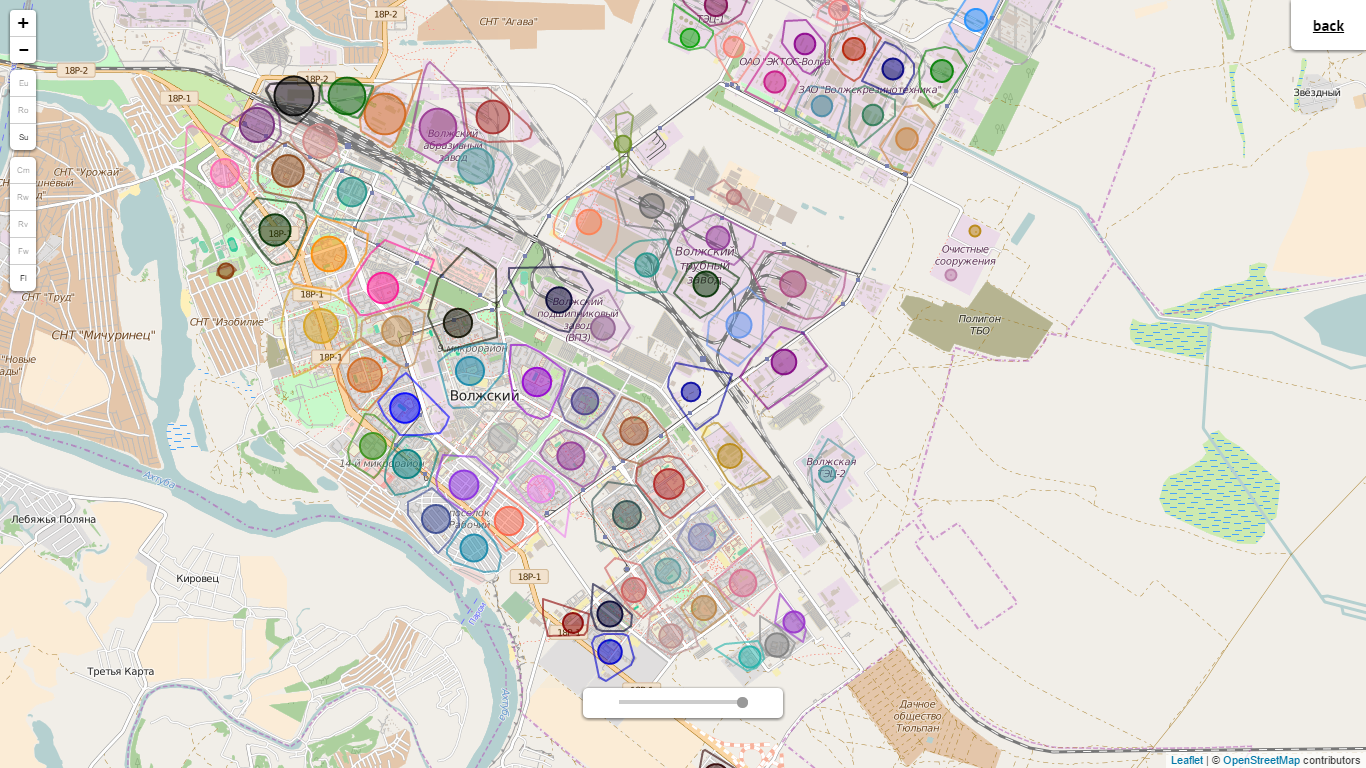
\includegraphics[width=.9\textwidth]{full_surface}
    \caption{Кластеризация выборки Main с метрикой Surface. Линиями очерчена выпуклая оболочка точек, принадлежащих кластерам. Круги~--- центры кластеров, радиус круга зависит от количества точек, принадлежащих кластеру.}
    \label{img:full-surface}
    \vspace*{-1ex}
\end{figure}

На рисунке~\ref{img:full-route} видно, что области, ограниченные линиями пересекаются. Это происходит из-за того, что при расчете расстояния сервис OSRM выбирает ближайшие к точкам участки дорожной сети, а затем строит маршрут по графу дорог между ними. Из-за этого точки, расположенные, например, по разные стороны одного дома попадают на разные участки дорог, и расстояние между ними и центром кластера получается различным.
\begin{figure}[t!]
    \centering
    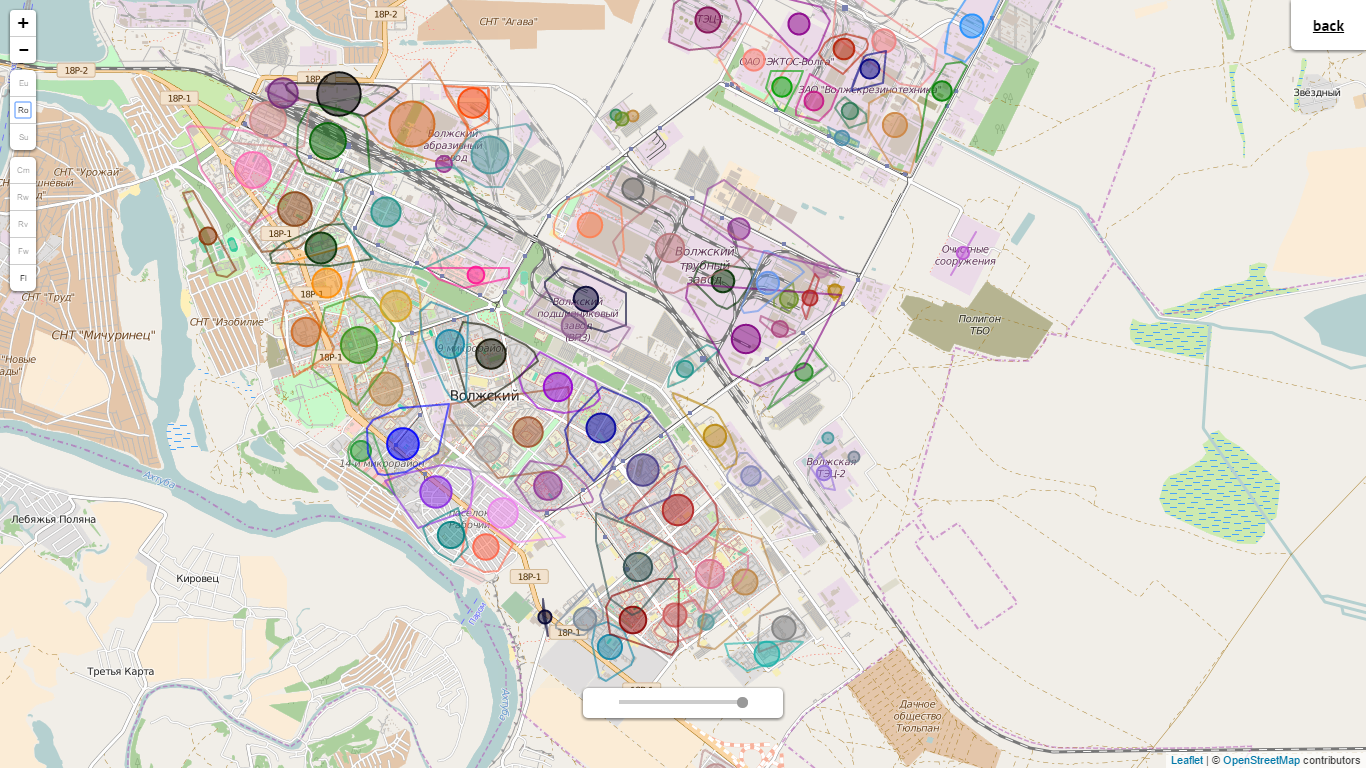
\includegraphics[width=.9\textwidth]{full_route}
    \caption{Кластеризация выборки Main с метрикой Route. Линиями очерчена выпуклая оболочка точек, принадлежащих кластерам. Круги~--- центры кластеров, радиус зависит от количества точек в кластере.}
    \label{img:full-route}
    \vspace*{-2ex}
\end{figure}

Для тестирования работы алгоритма расстановки остановочных пунктов использовалась часть выборки Main, детальный вид представлен на рис.~\ref{img:terminals}. Видно, что центры кластеров располагаются на участках дорожной сети.
\begin{figure}[b!]
    \vspace*{-1ex}
    \centering
    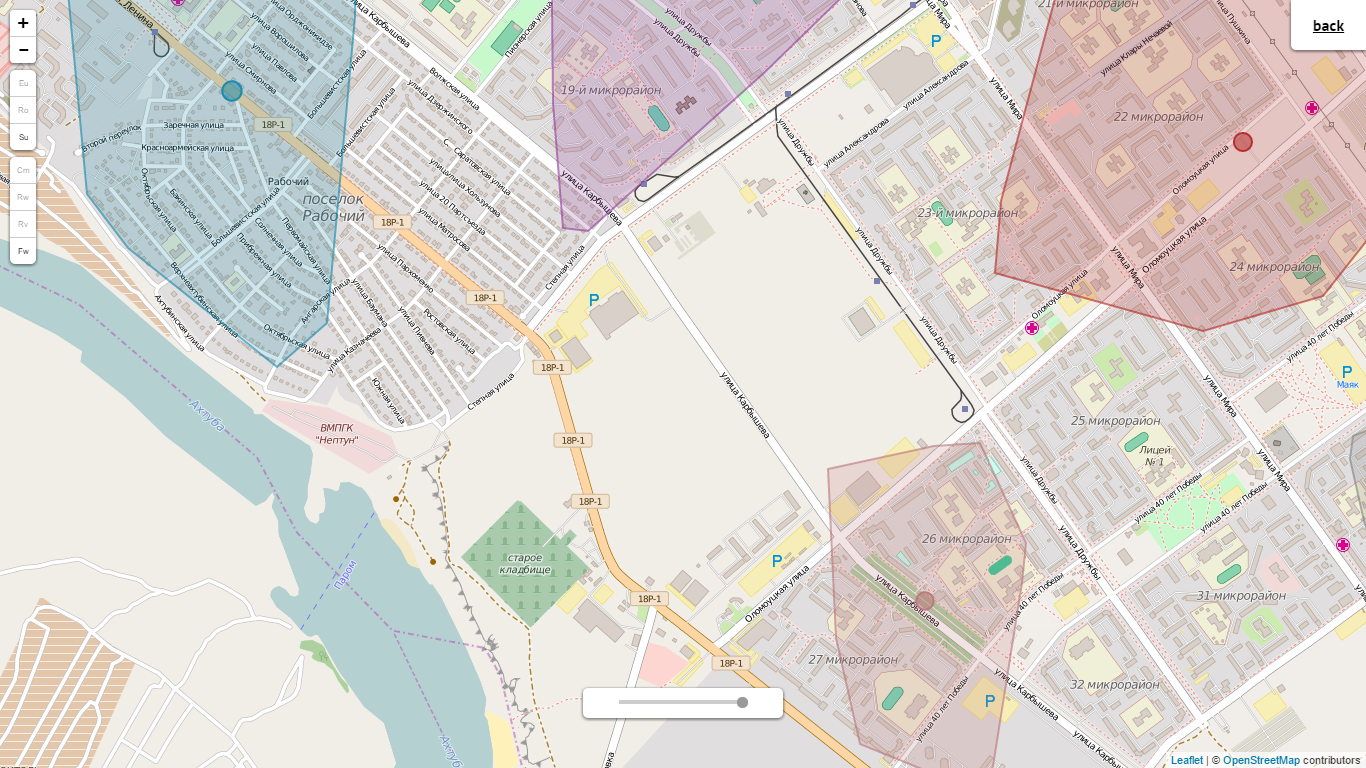
\includegraphics[width=.9\textwidth]{terminals}\\[1ex]
    \caption{Пример нахождения остановочных пунктов. Центры кластеров выделены кругами.}
    \label{img:terminals}
    \vspace*{-2em}
\end{figure}

\textbf{В четвертой главе} произведена оценка эффективности разработанных алгоритмов, были проведены эксперименты, в ходе которых менялись тестовые выборки, метрики расстояния, а также реализации данного метода.

Кластеризация выборки Main (1,5 млн расчетов дистанций) с метрикой Surface потребовала 28 итераций алгоритма. При использовании параллельной реализации (4 потока) на одну итерацию в среднем уходит по 17 минут. Кластеризация выборки Main с метрикой Route потребовала 21 итерацию алгоритма. При использовании параллельной реализации (4 потока) на одну итерацию в среднем уходит по 90 минут. Откуда можно сделать вывод, что на один расчет расстояния (при параллельной реализации) метрикой Surface уходит \( 0.66 \)~мсек, тогда как у метрики Route на это затрачивается \( 3.6 \)~мсек. Для сравнения, на один расчет Эвклидовой метрикой уходит \( 0.06 \)~мсек.

При непараллельной версии работы у метрики Surface в среднем на один расчет расстояния затрачивается \( 0.71 \)~мсек, у метрики Route~--- \( 4.8 \)~мсек. Для сравнения, на один расчет Эвклидовой метрикой уходит \( 0.07 \)~мсек.

\textbf{В заключении} работы сформулированы общие выводы по проделанной работе в рамках магистерской диссертации. Обсуждены полученные результаты и предложено направление для дальнейшего развития данной работы.

\textbf{В приложении} приведены материалы справочного характера и техническое задание на создание программы кластеризации географических точек для построения сети остановочных пунктов общественного транспорта.

\section{Основные результаты работы} В рамках магистерской диссертации был разработан метод кластеризации предпочтений жителей по перемещению, выраженных в форме пары геораспределенных объектов <<пункт отправления--пункт назначения>>. Для этого были использованы алгоритм кластеризации k-средних и метрика Route, рассчитывающая расстояния между геораспределенными объектами по графу дорог, для чего использующая сервис маршрутизации Open Source Routing Machine. Результаты работы алгоритма кластеризации используются для построения сети остановочных пунктов общественного транспорта.

\section{Перспективные направления развития работы}
Предложенный алгоритм может быть использован для построения сети остановочных пунктов общественного транспорта.
Разработанный модуль может быть использован как компонент системы формирования маршрутной сети городского транспорта.

\renewcommand{\bibname}{Публикации по теме диссертации}
\begin{thebibliography}{10}
    \bibitem{first} Strategway: web solutions for building public transportation routes using big geodata 
        analysis / Golubev A., Chechetkin I., Solnushkin K.S., Sadovnikova N., Parygin D., Shcherbakov M., 
        Brebels A. // Proceedings of The 17th International Conference on Information Integration and 
        Web-based Applications \& Services (iiWAS2015) (December 11 - 13, 2015 Brussels, Belgium) 
        ACM New York, New York pp. 665 - 668
    \bibitem{second} Комплекс инструментов интеллектуального анализа данных strategway для поддержки 
        принятия решений по управлению развитием инфраструктуры города / Садовникова Н.П., Щербаков М.В., 
        Парыгин Д.С., Солнушкин К.С., Голубев А.В., Чечеткин И.А. // В сборнике: Развитие средних 
        городов: замысел, модели, практика Материалы III Международной научно-практической конференции. 
        Волгоград, 2015. С. 147-150
    \bibitem{third} Автоматизация поддержки принятия решений по разработке маршрутов общественного 
        транспорта на основе анализа данных о корреспонденциях жителей / М. В. Щербаков, 
        Н. П. Садовникова, Д. С. Парыгин, А. В. Голубев, И. А. Чечеткин // Вестник компьютерных и 
        информационных технологий. -- М. : Издательский дом <<Спектр>>, 2016. -- Принята к печати.
\end{thebibliography}